\documentclass[letter,12pt,oneside]{report}
\usepackage[utf8]{inputenc}
\usepackage[spanish]{babel}
\usepackage{amsfonts}
\usepackage{amsmath}
\usepackage[pdftex]{graphicx}
\usepackage{url}
\usepackage[top=3cm,bottom=3cm,left=3cm,right=3cm,footskip=1.5cm,headheight=1.5cm,headsep=.5cm]{geometry}
\usepackage{datetime}
\usepackage{fancyhdr}
\usepackage[margin=1.5cm,font={small}]{caption}
\usepackage{setspace}
\usepackage{abstract}
\usepackage{float}
\usepackage[titles]{tocloft}
\usepackage{listings}
\usepackage{color}
\usepackage[T1]{fontenc}
\usepackage{txfonts}
\usepackage[breaklinks=true]{hyperref}
\usepackage{verbatim}
\usepackage{titlesec}
\titleclass{\subsubsubsection}{straight}[\subsection]

\newcounter{subsubsubsection}[subsubsection]

\renewcommand\thesubsubsubsection{\thesubsubsection.\arabic{subsubsubsection}}
\renewcommand\theparagraph{\thesubsubsubsection.\arabic{paragraph}}
\renewcommand\thesubparagraph{\theparagraph.\arabic{subparagraph}}

\titleformat{\subsubsubsection}
  {\normalfont\normalsize\bfseries}{\thesubsubsubsection}{1em}{}
\titlespacing*{\subsubsubsection}
{0pt}{3.25ex plus 1ex minus .2ex}{1.5ex plus .2ex}

\makeatletter
\renewcommand\paragraph{\@startsection{paragraph}{5}{\z@}%
  {3.25ex \@plus1ex \@minus.2ex}%
  {-1em}%
  {\normalfont\normalsize\bfseries}}
\renewcommand\subparagraph{\@startsection{subparagraph}{6}{\parindent}
  {3.25ex \@plus1ex \@minus .2ex}%
  {-1em}%
  {\normalfont\normalsize\bfseries}}
\def\toclevel@subsubsubsection{4}
\def\toclevel@paragraph{5}
\def\toclevel@paragraph{6}
\def\l@subsubsubsection{\@dottedtocline{4}{7em}{4em}}
\def\l@paragraph{\@dottedtocline{5}{10em}{5em}}
\def\l@subparagraph{\@dottedtocline{6}{14em}{6em}}
\@addtoreset{subsubsubsection}{section}
\@addtoreset{subsubsubsection}{subsection}
\@addtoreset{paragraph}{subsubsubsection}
\makeatother

\setcounter{secnumdepth}{6}
\setcounter{tocdepth}{6}

\hyphenation{con-fi-gu-ra-ción}
\hyphenation{ad-mi-nis-tra-dor}
\hyphenation{saw-zall}

\definecolor{dkgreen}{rgb}{0,0.6,0}
\definecolor{gray}{rgb}{0.5,0.5,0.5}
\definecolor{mauve}{rgb}{0.58,0,0.82}
\lstset{frame=tb,
  language=sql,
  aboveskip=0mm,
  belowskip=0mm,
  showstringspaces=false,
  columns=flexible,
  basicstyle={\ttfamily\scriptsize},
  numbers=none,
  numberstyle=\tiny\color{gray},
  keywordstyle=\color{blue},
  commentstyle=\color{dkgreen},
  stringstyle=\color{mauve},
  breaklines=true,
  breakatwhitespace=true
  tabsize=3
}
\setlength{\parskip}{0.1cm}
\hypersetup{%
  colorlinks=false,% hyperlinks will be black
  pdfborderstyle={/S/U/W 0}% border style will be underline of width 1pt
}
\newenvironment{dedication}
{
   \cleardoublepage
   \vspace*{\stretch{8}}
   \hfill\begin{minipage}[t]{0.66\textwidth}
   \raggedright
}%
{
   \end{minipage}
   \clearpage
}
\fancypagestyle{fancyplain}{
\renewcommand{\headrulewidth}{0pt}
\fancyhf{}
\fancyfoot[R]{\thepage}
}
\fancyhf{}
\lhead{\leftmark }
\fancyfoot[C]{\thepage}
\pagestyle{fancy}
\renewcommand{\chaptermark}[1]{\markboth{\MakeUppercase{\chaptername\ \thechapter\ :\ #1}}{}}
\addto\captionsspanish{%
  \renewcommand\listfigurename{Índice de Figuras}
  \renewcommand\listtablename{Índice de Tablas}
  \renewcommand\refname{Referencias Bibliográficas}
  \renewcommand{\tablename}{Tabla}
  \renewcommand{\cftfigfont}{Figura }
  \renewcommand{\cfttabfont}{Tabla }
  }

\renewcommand{\arraystretch}{1.5}
\renewcommand{\baselinestretch}{1.50}\normalsize
\renewcommand{\abstractnamefont}{\normalfont\Large\bfseries}
\renewcommand{\abstractname}{Agradecimientos}
\newcommand{\quotes}[1]{``#1''}
\begin{document}
\begin{titlepage}
\center 
\Large{UNIVERSIDAD TÉCNICA FEDERICO SANTA MARÍA}\vspace{-2mm}  % Name of your university/college
\large{DEPARTAMENTO DE INFORMÁTICA}\\\vspace{-1mm} % Major heading such as course name
\normalsize{SANTIAGO - CHILE}\\\vspace{5mm} % Minor heading such as course title

\includegraphics[height=125px]{images/ISOTIPO-Color.jpg}\\\vspace{15mm} % Include a department/university logo - this will require the graphicx package
\LARGE{\textsc{Análisis en Base de Inteligencia de Negocios para las fallas en terminaciones en la industria de la construcción en Chile}}\vspace{18mm}\\
\large{PAULINA AGUILA BUSTOS}\\\vspace{10mm}  % Name of your university/college
\normalsize{MEMORIA DE TITULACIÓN PARA OPTAR AL TÍTULO DE\\ INGENIERO CIVIL EN INFORMÁTICA}\\\vspace{12mm}
%\begin{minipage}{0.4\textwidth}
%\begin{flushleft}
\normalsize{\textsc{PROFESOR GUÍA: José Luis Martí Lara}}\\\vspace{13mm}
%\textbf{\small{PROFESOR CORREFERENTE:}}
%\end{flushleft}
%\end{minipage}
%~
%\begin{minipage}{0.5\textwidth}
%\begin{flushright}
%\small{José Luis Martí Lara}\\
%\textbf{\small{PROFE CORREFERENTE}}
%\end{flushright}
%\end{minipage}

\large{septiembre - 2016}%trampa, modificar fechas es un cacho
\vfill % Fill the rest of the page with whitespace
\end{titlepage}
\newpage
\thispagestyle{fancyplain}
\pagenumbering{roman}
\setcounter{page}{1}
\begin{comment}
\newpage
\thispagestyle{fancyplain}
\section*{Agradecimientos}
Me gustaría agradecer a Mi.
\newpage 
\thispagestyle{fancyplain}
\begin{dedication}
Este documento está dedicado a xxssdd\\
\end{dedication}
\newpage
\thispagestyle{fancyplain}
\renewcommand{\abstractnamefont}{\normalfont\Large\bfseries}
\renewcommand{\abstractname}{Resumen}
\begin{abstract}
Abstracto\\
{\textbf{Palabras Clave:}} 
\end{abstract}
\renewcommand{\abstractname}{Abstract}
\begin{abstract}
Abstracto \\
{\textbf{Keywords:}} 
\end{abstract}
\end{comment}
\newpage
\renewcommand{\contentsname}{Índice General}
\tableofcontents
\listoffigures
%\listoftables

%	INTRODUCCIÓN	---------------------------------------------------------------------------------------------------------------------------
\newpage
\thispagestyle{fancyplain}
\chapter{Introducción}
Para la realización de la memoria, se trabajará con una empresa llamada RyR Optimiza que lleva más de 5 años en la industria del desarrollo de software. Ellos trabajan en el área de la construcción de viviendas en Chile y pronto se abrirán a otros países sudamericanos.

La empresa RyR, tiene un software o sitio web llamado CalidadCloud, el cual consta de distintos módulos que corresponden a las diversas etapas de la construcción de propiedades, desde la inscripción de proyectos, pasando por obra gruesa y hormigón, verificando la calidad de lo construido y finalizando en la recepción de la vivienda revisando las terminaciones.

Es en este último módulo en el que se centrará la memoria a realizar, el cual se llama “Recepciones”, el cual actualmente consta con cientos de miles de datos, los que están estandarizados para todas las empresas. Con esta gran cantidad de datos, es posible realizar un análisis basándose en Inteligencia de Negocios que tenga la suficiente validez.

En Recepciones existen fichas para cada propiedad, dentro de las fichas se tienen recintos, que pueden ser: baños, dormitorios, cocina, terraza, entre otras. Los recintos tienen a su vez lugares, que para el caso de un baño puede ser: tina, ducha, lavamanos, espejo, etc. Finalmente, dentro del lugar se encuentran los ítems, que es el último detalle. Los ítems para el lugar tina podrían ser: llave, loza, tapón, etc. Cada ítem se revisa con estados de cumple, falla o no aplica. En el caso de falla, se debe especificar el por qué falla, teniendo una serie de opciones como: manchado, roto, falta pieza, y varios más. Se tiene que al solucionar la falla, ésta debe ser marcada como solucionada.

La memoria estará enfocada en utilizar Inteligencia de Negocios para crear un Data Warehouse y por medio de análisis OLAP poder obtener las fallas y detalles de fallas más comunes en Chile, analizando también variables como el piso (en caso de departamentos), ubicación del proyecto, tiempo promedio de solución de fallas, entre otras cosas.

Al tener el análisis finalizado, se espera realizar una actualización a la aplicación móvil de Recepciones que genere una especie de alerta al momento de inspeccionar la vivienda, de tal forma que en base a los datos estadísticos obtenidos anteriormente, se pueda conocer la probabilidad de que cierto recinto/lugar/ítem pueda fallar, lo que alertaría antes al usuario para que revise con más cautela.

Se espera poner en práctica esta alerta durante un tiempo, para luego conocer si realmente le fue de ayuda al momento de revisar la propiedad. Estos resultados serán la última etapa de la memoria que se realizará en un tiempo máximo de 4 meses.

El presente trabajo constará con la siguiente estructura:

\begin{itemize}
\item \textbf{Capítulo 2: Definición del Problema.} En esta sección se hará una breve descripción de la empresa con la que se trabajará y la importancia de realizar este trabajo. Acá es donde se definirán los objetivos que se esperan cumplir en su totalidad al finalizar la memoria.
\item \textbf{Capítulo 3: Estado del Arte.} En este capítulo se realiza una profunda investigación de los elementos básicos que componen la solución a desarrollar, como es principalmente la Inteligencia de Negocios y la Tecnología Móvil.
\item \textbf{Capítulo 4: Diseño de la Solución.} En esta sección se diseña la solución, así como la definición de las variables que responden los objetivos y una explicación completa y detallada de los datos a analizar. Se desarrolla un modelo multidimensional que cumpla con lo requerido.
\item \textbf{Capítulo 5: Construcción e Implementación de la Solución.} En este capítulo se detalla la construcción de la solución diseñada en la sección anterior, detallando la metodología y herramientas con que se construirá y posteriormente su implementación en la aplicación móvil.
\item \textbf{Capítulo 6: Análisis y Resultados.} En esta sección se revisan y analizan los resultados de la implementación y de la solución en detalle.
\item \textbf{Capítulo 7: Conclusión.} En este último capítulo, se detalla el cumplimiento de los objetivos y una síntesis del trabajo realizado y de los resultados obtenidos.
\end{itemize}

%	DEFINICIÓN DEL PROBLEMA	-----------------------------------------------------------------------------------------------------------
\newpage
\pagenumbering{arabic}
\thispagestyle{fancyplain}
\chapter{Definición del Problema}

\section{Descripción de la Empresa}
R\&R Optimiza\footnote{\url{http://www.ryroptimiza.cl/}} es una empresa que tiene 4 años de experiencia dedicándose a innovar en el área de la gestión en construcción, cuyo compromiso es entregar a las organizaciones herramientas que permitan mejorar sus procesos mediante soluciones simples e innovadoras a través de tecnologías informáticas con el fin de orientarlos en un proceso de mejora continua.

En la actualidad, R\&R cuenta con dos softwares principales, uno es Calidad Cloud y el otro es Laboral Box\footnote{Laboral Box, es un sistema que permite controlar toda la documentación de los RRHH dentro de las empresas, facilitando la gestión de control. \url{http://www.ryroptimiza.cl/\#!laboral-box/jz7rt}}. Calidad Cloud es un sistema digital que permite controlar los procesos de construcción que se llevan a cabo en obras. Las listas de chequeo que comúnmente se realizan de forma manual, en CCloud se realizan digitalmente, lo que permite realizar análisis comparativos en tiempo real de lo que sucede en la obra, ahorrándose el tiempo de traspasar la información a un sistema informático.

CCloud se compone de una serie de módulos que manejan los diversos procesos de construcción. Los módulos son: Hormigón, Calidad, Indicadores, Recepción y Entregas. Los módulos de Calidad y de Recepciones poseen su versión en aplicación móvil, lo que permite a los usuarios ingresar información en terreno para luego sincronizarlas con las existentes.

El módulo de Recepciones permite recolectar información sobre las terminaciones de los diversos recintos, lugares e ítems dentro de una propiedad. En este caso, los recintos corresponden a los sectores generales que componen la vivienda, como son: dormitorios, baños, cocina, terraza, entre otros. Por otro lado, los lugares están dentro de los recintos y son elementos que lo componen, por ejemplo, para el recinto cocina, se tienen lugares como: campana de extracción, horno empotrado eléctrico, lavaplatos, etc. Finalmente, los ítems son elementos que componen los lugares, por ejemplo, ítems que tiene el lugar horno empotrado eléctrico dentro de la cocina serían: ampolleta, bandeja, enchufe, puerta, entre otros.

\section{Descripción del Problema}
En la actualidad, es muy importante para las empresas poder tomar control de la información que almacenan sobre sus clientes, por lo que realizar un análisis detallado de su información es primordial.

En Chile, no se han realizado análisis completos de las terminaciones a nivel de la construcción en los últimos años, por lo que sería interesante dar a conocer a las empresas constructoras e inmobiliarias lo que ocurre al finalizar sus obras.

Existen muchas herramientas que permiten analizar desde muchos puntos de vista un gran volumen de datos utilizando Inteligencia de Negocios, por lo que no hacer un estudio de los datos almacenados hace que la empresa pierda ventaja competitiva y evita que se conozcan datos estadísticos que muestren los problemas actuales de las constructoras chilenas.

Por otro lado, las tecnologías móviles están entrando cada vez más fuerte en las empresas, y el unir dos potenciales herramientas como son las aplicaciones móviles y la inteligencia de negocios en un solo producto añadiría mucho más valor al producto y, por ende, a la empresa, lo que la haría crecer mucho más.

Otra utilidad de analizar los datos de las terminaciones recopilados en el módulo de Recepciones, sería en el módulo de Calidad, en donde se podría prestar una mayor atención a los sectores que tienen más fallas en las terminaciones, lo que haría que disminuyeran los errores en las futuras construcciones. Sin embargo, esto sería para un trabajo futuro, ya que actualmente, el módulo de Calidad no está estandarizado, por lo que los datos se deben someter a un proceso de transformación y estandarización para poder utilizarlos para análisis. Este es un proceso que se espera que se realice en los próximos meses.

\section{Objetivos}
\subsection{Objetivo Principal}
Se debe diseñar y construir un modelo multidimensional de Inteligencia de Negocios que permita responder y entregar relaciones entre las distintas variables que se analizarán para las terminaciones de propiedades, con la finalidad de conocer el estado actual en la industria.

\subsection{Objetivos Específicos}
\begin{itemize}
\item Se deben identificar las variables más importantes que logren explicar el comportamiento de la construcción en la industria chilena.
\item Se debe construir un modelo multidimensional con las variables escogidas y realizar un análisis OLAP sobre ellos.
\item Una vez teniendo la información detallada y los resultados del análisis OLAP, se actualiza la aplicación móvil Recepciones añadiendo alertas que permitan informar al usuario de posibles fallas cuando éste vaya a inspeccionar.
\item La aplicación actualizada se pone en práctica durante un tiempo y se analizan los resultados y opiniones de los usuarios.
\end{itemize}

%	ESTADO DEL ARTE	----------------------------------------------------------------------------------------------------------------------
\newpage
\chapter{Estado del Arte}

\section{Inteligencia de Negocios}
\subsection{Contexto}
Actualmente, las empresas suelen ser muy competitivas entre sí, por lo que diferenciarse de las demás es una tarea bastante complicada. Una ventaja competitiva de cierta empresa sobre otra del mismo rubro, sería conocer de mejor manera a sus clientes, de tal forma que se les ofrezcan cosas que a ellos les interese. Otro tipo de ventaja, sería conocer las fluctuaciones de ciertos indicadores que le permitan a la organización tomar mejores decisiones para el futuro. Estos tipos de análisis, requieren de ciertas herramientas que permitan obtener información a partir de los datos en bruto.

La Inteligencia de Negocios, también conocida como BI (Business Intelligence), es una combinación de tecnologías, herramientas y procesos que ayudan a la toma de decisiones de diferentes organizaciones. Con esta herramienta, se pueden aprovechar los datos almacenados en bases de datos por ciertas aplicaciones empresariales, ajustándolos para obtener la información que cubra el área de interés que se desea analizar \cite{P2}.

Las organizaciones almacenan datos provenientes de la interacción de sus clientes con los programas computacionales o los sitios web, pero estos datos por sí solos no tienen ninguna relevancia. Para obtener información a partir de los datos, estos se deben procesar y organizar de tal forma que se pueda realizar un análisis de ellos. El conocimiento, surge de un conjunto de información que se haya almacenado a través del tiempo o de análisis anteriores, el cual se puede crear y administrar a través de BI.

Las herramientas de BI pueden ser utilizadas a distinta escala dentro de una organización, ya sea para áreas específicas de la empresa o para todas las áreas, todo esto depende de los recursos que se tengan para implementar BI, y también de lo que se desea obtener como resultado, de igual forma se logrará una mejora en la eficiencia de los procesos y con ello una ventaja competitiva. 

\subsection{Componentes de Inteligencia de Negocios}
La inteligencia de negocios está compuesta por una serie de elementos que permiten transformar los datos a información realmente útil. Estos elementos son parte de un proceso que se debe llevar a cabo en su totalidad al aplicar BI a un conjunto de datos (dataset). La figura \ref{bi_comp} muestra estos elementos y la relación entre ellos.

\begin{figure}[h]
\begin{center}
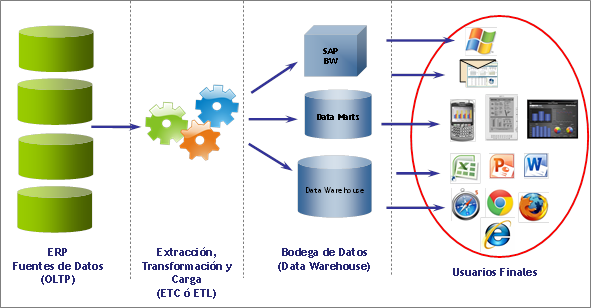
\includegraphics[scale=0.8]{images/bi_components.png}
\caption{Elementos que componen la Inteligencia de Negocios.}
\text{Fuente: \cite{U3}}
\label{bi_comp}
\end{center}
\end{figure}

\subsubsection{Fuentes de Datos}
Para comenzar a utilizar BI dentro de una organización, se debe contar con datos iniciales, los cuales pueden proceder de sistemas OLTP (On-line Transactional Processing) que se conocen como bases de datos, planillas de cálculo, sistemas ERP\footnote{ERP: Enterprise Resource Planning. Son sistemas de planificación de recursos empresariales.} o CRM\footnote{CRM: Customer Relationship Management} \cite{P3}. Estos serán los datos que se analizarán posteriormente para satisfacer los objetivos deseados, además, es muy importante que estos datos a utilizar sean de la mayor calidad posible, por lo que las fuentes de datos deben ser de gran confianza y estar totalmente documentadas. Las fuentes pueden ser de procedencia interna o externa a la organización.

\subsubsection{ETL}
Otro proceso importante de la aplicación de BI es la Extracción, Transformación y Carga, conocido como ETC o ETL\footnote{ETL: Extract, Transform and Load}. Es un proceso que no es visible para los usuarios finales, sin embargo, es muy importante realizarlo, ya que entregará la materia prima con la que se construirán los datos finales a analizar (\textit{Data Warehouse}). El detalle de cada elemento que lo compone se describe a continuación:

\begin{itemize}
\item\textbf{Extracción:} Este proceso corresponde a la extracción de los datos desde distintas fuentes de datos, como son bases de datos, planillas de cálculo, datos provenientes de programas ERP o CRM, entre otras.
\item \textbf{Transformación:} Corresponde a la etapa en donde se unen los datos extraídos de las diversas fuentes, por lo que es el proceso de mayor dificultad, ya que los datos no siguen un estándar y los conceptos pueden variar entre las fuentes. Otro problema, es que algunos datos poseen valores con errores que disminuyen la calidad de los datos finales. Para esta etapa se necesita una gran cantidad de tiempo. Los datos se almacenan en un área intermedia llamada \textit{Staging Area}.
\item \textbf{Carga:} Una vez que los datos están completamente estandarizados y sin errores, estos son transportados al área de almacenamiento principal llamada \textit{Data Warehouse}.
\end{itemize}

\subsubsection{Data Warehouse}
El Data Warehouse, desde ahora DW, es el almacén que contiene los datos provenientes del proceso ETL que se utilizarán para hacer los futuros análisis. Este almacén cumple con una serie de características \cite{P4}:

\begin{itemize}
\item\textbf{Temático: }En el DW solo se almacenarán los datos que generen conocimiento y sean de importancia para los objetivos que se deseen lograr. Para un mejor entendimiento de los datos por parte de los usuarios finales, los datos de la misma temática se deben albergar en una misma tabla, para facilitar su acceso y tiempo de búsqueda. Por ejemplo, al tratarse de fallas, éstos deben estar en una tabla en donde se unan todos los tipos de fallas que se describen en los datos.
\item\textbf{Integrado: }Los datos almacenados en el DW deben ser consistentes entre sí, por lo que deben haber pasado previamente por el proceso ETL. Además, deben tener la granularidad necesaria para satisfacer los objetivos esperados.
\item\textbf{No volátil: }No se pueden modificar los datos históricos que se hayan almacenado anteriormente en el DW, sino que solo se permite la inserción de los nuevos datos que hayan sido agregados al entorno operacional, lo que significa que el DW está hecho para ser leído y analizado, no para ser modificado.
\item\textbf{Histórico: }Los datos contenidos en el DW corresponden a datos históricos y actuales, lo que permite hacer análisis de tendencias y fluctuaciones de distintas variables, pudiendo comparar los resultados a través del tiempo. 
\end{itemize}

\subsubsection{Data Mart}
Los Data Mart (DM) son ``mercados de datos”, y generalmente, corresponden a subconjuntos de los DW. Están enfocados a distintas áreas del negocio, divisiones o departamentos de la organización, entre otras. Su finalidad, es ayudar a la toma de decisiones en dichos subconjuntos de forma similar a los DW, pero a una escala menor y de forma más particular.

Dentro de los DW, se pueden ver los DM como dimensiones dentro de un cubo multidimensional que permiten analizar los datos desde diferentes puntos de vista.

\subsubsection{OLAP}
Los OLAP (\textit{On-line Analytical Processing}), son análisis multidimensionales en base a las tablas y dimensiones tanto de los DW como de los DM. Las operaciones OLAP permiten que los usuarios finales puedan analizar los datos a través de herramientas computacionales que facilitan la interacción entre las dimensiones del DW. 

Este tipo de análisis permite realizar ciertas operaciones analíticas con los datos, como por ejemplo, listar ranking con los productos más vendidos en cierto negocio, agrupar los datos por valores específicos, y una interfaz en donde se observan las tendencias estudiadas. Las funcionalidades principales de estas herramientas OLAP, son la agrupación y agregación. En la figura \ref{olap} se puede ver una representación multidimensional en forma de cubo de los datos.

\begin{figure}[h]
\begin{center}
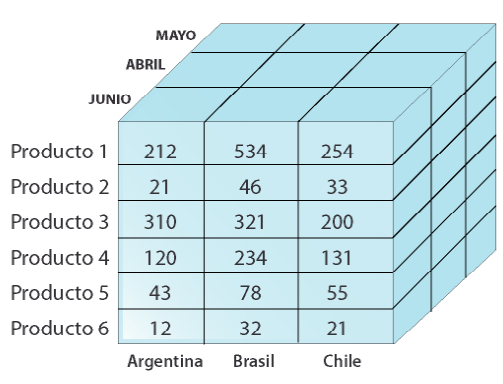
\includegraphics[scale=0.6]{images/olap.png}
\caption{Datos de un DW mostrados en forma cubo multidimensional.}
\text{Fuente: \cite{P3}}
\label{olap}
\end{center}
\end{figure}

\subsubsection{Data Mining}
La minería de datos, es el proceso de descubrir el conocimiento, lo que se logra moviéndose a través de los datos y analizándolos en busca de patrones y correlaciones entre variables que puedan guiar la toma de decisiones. Los modelos finales de minería de datos pueden ser resultados parciales y no lo que se espera, teniendo que volver a mover las variables para lograr lo deseado.

Para comenzar con minería de datos, se debe plantear una pregunta inicial que se espera responder en base a variables y dimensiones, para las cuales se deben establecer indicadores que logren responder las preguntas planteadas.

La minería de datos puede guiarse en dos caminos distintos dependiendo de lo que se espera lograr. Se pueden realizar análisis descriptivos y modelos predictivos. Los primeros tienen como finalidad describir los datos y establecer relaciones entre las variables en caso de existir, mientras que los modelos predictivos deben predecir el comportamiento de ciertas variables en base a otras, esto basándose en datos históricos. Los modelos predictivos son más complejos de desarrollar, ya que existen diversas técnicas de distinta dificultad y en su mayoría requieren conocimiento estadístico y de análisis computacional.

\subsubsection{Dashboards}
Los dashboards, son despliegues visuales de los análisis OLAP mostrados en variadas vistas y gráficos, todo esto en una sola ventana. La figura \ref{dashboard} muestra un ejemplo de dashboard.

Son muy utilizados en todas las áreas de las organizaciones debido a su forma concisa y resumida de mostrar la información en tiempo real, permitiendo realizar análisis instantáneos del negocio apoyando la toma de decisiones. También se utilizan como forma de presentar información en reuniones sobre las tendencias de la empresa.

\begin{figure}[h]
\begin{center}
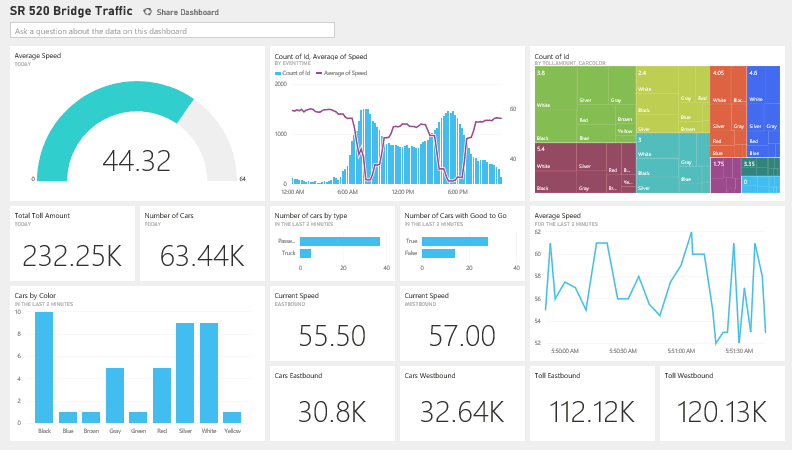
\includegraphics[scale=0.5]{images/dashboard.png}
\caption{Datos de un DW mostrados en forma cubo multidimensional.}
\text{Fuente: \url{http://www.bi-it.com.mx/dashboard.html}}
\label{dashboard}
\end{center}
\end{figure}

\subsection{Construccion del DW}
Para la construcción de un DW que contenga los datos necesarios para cumplir con los objetivos deseados, existen diversas metodologías de BI que lo hacen posible. En este caso, se utilizará la metodología de Kimball \cite{P4}, la cual es actualmente la más usada.

Esta metodología, contempla una serie de pasos previos a la construcción del modelo multidimensional, sin embargo, en esta sección solo se describirán los pasos para el modelado dimensional, asumiendo que ya se tiene el área de negocio a analizar claramente definido.

Ralph Kimball, propone un modelo compuesto de Hechos y Dimensiones, en donde los Hechos serán los objetos a analizar y las Dimensiones serán los puntos de vista con los que se podrán analizar los Hechos. Estos últimos, se representarán como medidas o indicadores, mientras que las dimensiones quedan representadas como conjunto de atributos \cite{P5}.

Los hechos, corresponden a las tablas en las que se basarán los analistas para tomar las decisiones. Estas pueden ser filtradas, agrupadas y analizadas en base a las dimensiones. 

La representación utilizada para este tipo de DW, es un cubo o hipercubo multidimensional, dependiendo de la cantidad de atributos y dimensiones que se tengan. La intersección de los ejes contendrá los valores de los Hechos o de los indicadores a evaluar. Esto se aprecia en la Figura \ref{olap}.

En estos cubos multidimensionales, se pueden tener los siguientes objetos:

\begin{itemize}
\item \textbf{Atributos: }Pertenecen a las tablas de dimensiones y se refieren a los criterios en que se basarán los análisis.
\item \textbf{Indicadores: }Agregación o sumarización sobre valores de las tablas de Hecho.
\item \textbf{Jerarquías: }Relaciones lógicas que puedan existir entre diversos atributos.
\end{itemize}

El proceso de diseño comienza con un modelo dimensional de alto nivel obtenido a partir de los procesos priorizados, el cual consta de 4 pasos:

\begin{enumerate}
\item\textbf{Elegir el proceso de negocio: }Elección del área a modelar. Corresponde a una decisión de la dirección y cargos superiores. Los datos a utilizar deben estar contenido de alguna forma en un tipo de repositorio o base de datos. De esta elección dependerán todos los pasos siguientes, por lo que se debe hacer correctamente. 
\item\textbf{Establecer el nivel de granularidad: }En esta etapa, se debe especificar el nivel de detalle. La elección de la granularidad depende de los requerimientos del negocio y de los datos actuales. La sugerencia general es comenzar a diseñar el DW al mayor nivel de detalle posible, ya que se podría luego realizar agrupamientos al nivel deseado. En caso contrario no sería posible abrir (drill-down) las sumarizaciones o agrupaciones, ya que el nivel de detalle no lo permitiría. Sin embargo, tener mucho nivel de detalle también haría que las consultas fueran más lentas.
\item\textbf{Elegir las dimensiones: }Las dimensiones surgen de las discusiones del equipo, y facilitadas por la elección del nivel de granularidad y de la matriz de hechos/dimensiones. Las tablas de dimensiones tienen un conjunto de atributos (generalmente textuales) que brindan una perspectiva o forma de análisis sobre una medida en una tabla de hechos. 
\item\textbf{Identificar las tablas de hechos y medidas: }El último paso consiste en identificar las medidas que surgen de los procesos del negocio. Una medida es un atributo (campo) de una tabla que se desea analizar, sumarizando o agrupando sus datos, usando los criterios de corte conocidos como dimensiones. Las medidas se vinculan al nivel de granularidad y se encuentran en las tablas de hechos, en donde, cada una de ellas tiene como atributos una o más medidas de un proceso organizacional, de acuerdo a los requerimientos.
\end{enumerate}

\section{Tecnologia Móvil}
\subsection{Evolución y Uso en Empresas}
En los tiempos actuales, la tecnología móvil es una herramienta fundamental para el desarrollo de las actividades profesionales y cotidianas de las personas. La conectividad a través de las redes 4G ha permitido tener acceso a una infinidad de conocimiento en tiempo real desde cualquier lugar del mundo. Las personas adoptan estas tecnologías cada vez más rápido, haciéndolas parte fundamental de sus vidas\cite{P6}.

La mayoría de las empresas de cualquier rubro, utilizan alguna tecnología móvil con la finalidad de agilizar los procesos que anteriormente se hacían de forma manual. Con esto han disminuido sus gastos y los tiempos de ejecución de ciertas tareas \cite{P1}. Es muy difícil imaginar y recordar cómo se realizaban dichas acciones en el pasado, el tener que llegar a un lugar establecido para poder leer los correos electrónicos, interactuar con personas a la distancia o simplemente leer sobre noticias internacionales. Ahora, todo eso se puede hacer de forma instantánea gracias a la evolución que ha tenido la tecnología móvil.

A esto también se le suma la evolución de los aparatos móviles, desde la aparición del llamado “celular” que utilizaba señales 1G que solo le permitía realizar conexiones de voz, teniendo una configuración muy básica. Luego, se lanzó la tecnología 2G que mejoró considerablemente la calidad de las llamadas de voz, añadiendo además los populares SMS\footnote{SMS: Short Message Service (Servicio de Mensajes Cortos)}. La llegada del 3G revolucionó todas las formas conocidas de conectividad móvil, permitiendo el acceso al mundo web a una gran velocidad desde cualquier lugar, posibilitando el desarrollo continuo e imparable de las aplicaciones móviles. Finalmente, con el 4G se alcanza una cobertura casi total, que llega hasta los lugares más alejados y permitiendo una velocidad de transmisión de datos que se compara con la fibra óptica.

Toda esta evolución, permitió a las empresas comenzar a desarrollar aplicaciones móviles con la finalidad de que sus clientes pudiesen tener acceso a sus productos de forma instantánea facilitando su acceso.

Según un estudio realizado por la IDC\footnote{International Data Corporation. \url{http://www.idc.com/}}\cite{U2}, informó que las aplicaciones móviles más utilizadas por las empresas son las llamadas CRM, que tienen como finalidad almacenar la mayor cantidad posible de datos de los clientes para así poder conocer lo que ellos prefieren y entregarles información que ellos aprecien. Por otro lado, las aplicaciones basadas en Inteligencia de Negocios también están siendo muy demandas, para los empresarios es fundamental conocer los caminos que van siguiendo sus indicadores en tiempo real. Finalmente, otro tipo de aplicaciones que es muy demandado, son las que permiten el almacenamiento de datos en la nube, de forma de tener acceso a él desde cualquier lugar, otro motivo para esto, es que los datos almacenados por las empresas crecen de forma exponencial, por lo que los espacios libres son cada vez más escasos, siendo buena idea este tipo de almacenamiento.

%	DISEÑO DE LA SOLUCIÓN		-----------------------------------------------------------------------------------------------------------
\newpage
\chapter{Diseño de la Solución}

\section{Identificación de variables relevantes}
En primer lugar, se debe tener en cuenta que los usuarios que tendrán acceso a los resultados del análisis, tendrán un perfil técnico enfocado en la calidad de la construcción, por lo tanto, los resultados que ellos deben observar, tienen que presentarse de tal forma que ellos lo comprendan fácilmente, sin utilizar lenguajes que no pertenecen a su rubro. Estas personas están encargadas de revisar las terminaciones de los proyectos, es decir, verificar que cada recinto cumpla con las especificaciones de calidad establecidas por la empresa.

En base a dicho perfil, es necesario identificar las variables del problema que les permita a los usuarios poder conocer el estado de las viviendas de forma global, pudiendo tener un conocimiento más amplio sobre las tareas específicas que están fallando en todo el proyecto.

\subsection{Especificaciones de Requerimientos}
Para los usuarios descritos, es interesante poder obtener la siguiente información a través del análisis:

\begin{itemize}
\item \textbf{Cuáles son los recintos, lugares e ítems que fallan constantemente.} Hasta el momento, los usuarios solo pueden filtrar por estados de una propiedad, pero no tienen una estadística general sobre las fallas en todo el proyecto. Este análisis los podría ayudar a tener una visión global sobre lo que ocurre en la obra.
\item \textbf{Tipos de fallas más frecuentes, de forma global y por recinto, lugar e ítem.} Sería importante conocer cuáles son los tipos de fallas que se encuentran de forma frecuente en los proyectos. Por ejemplo, si el resultado entregara que en el baño hay más fallas del tipo “humedad”, los encargados podrían comenzar una investigación para conocer las causas.
\item \textbf{Conocer la cantidad de fallas por piso, en el caso de edificios.} Este sería un análisis que permitiría conocer si existe algún aprendizaje por parte de los trabajadores al conocer las fallas de los primeros pisos, procurando no volver a cometerlas en los pisos superiores.
\end{itemize}

En general, el proceso de negocio que se debe modelar y que cubre los tres requerimientos detallados, es el análisis de fallas, lo que se aplicará a distintas variables del problema.

\subsection{Dimensiones}
Las variables de datos que permiten satisfacer los requerimientos especificados, son las siguientes:

\begin{itemize}
\item \textbf{Recintos: }Variable categórica nominal que contiene el nombre del recinto que posee una propiedad. Una propiedad tiene múltiples recintos.
\item \textbf{Lugares: }Variable categórica nominal que contiene el nombre del lugar que posee un recinto de una propiedad. Un recinto tiene múltiples lugares.
\item \textbf{Items: }Variable categórica nominal que contiene el nombre del ítem que posee un lugar de un recinto de una propiedad. Un lugar tiene múltiples ítems.
\item \textbf{Piso: }Variable cuantitativa continua que representa el piso en donde se encuentra la propiedad. Toma valores dependiendo la cantidad de pisos del edificio de cada proyecto. Para proyectos de casas, esta variable no aplicará.
\item \textbf{Estado: }Variable categórica nominal que representa el estado de la revisión. Puede tomar los siguientes valores: Cumple, Falla, No Aplica y Solucionado.
\item \textbf{Tipo de Falla: }Variable categórica nominal que contiene el nombre de la falla del ítem en caso de que el estado de revisión sea “falla”. Puede tomar una serie de valores registrados en la base de datos.
\item \textbf{Origen: }Variable categórica de tipo nominal que representa el dispositivo en donde se realizó la revisión. Puede tomar los siguientes valores: Webapp: para el caso en que se revisó a través de la web - Móvil: cuando se revisó en un teléfono móvil.
\end{itemize}

\section{Fuentes de Datos}
Los datos se obtuvieron directamente desde la aplicación Calidad Cloud, la que contiene el módulo de Recepciones, el cual tiene los datos de las revisiones de terminaciones de las propiedades. 

Se trabajará con datos provenientes de 11 empresas constructoras distintas, con la finalidad de abarcar gran parte de la industria chilena, y que los resultados de los análisis puedan ser más generales y globales. Estos datos fueron facilitados por la empresa R\&R Optimiza y corresponden a archivos .csv con todas las variables necesarias para responder de forma correcta los requerimientos especificados.

\section{Modelo Lógico}
Como se pudo ver en la sección 4.1.1, el proceso de negocio a modelar es el Análisis de Fallas en las terminaciones de las propiedades aplicado a las diversas dimensiones de los datos.

Para la construcción del DW, se toman en cuenta todas las dimensiones que satisfacen el problema y sus relaciones, creando el modelo relacional que se muestra en la Figura \ref{rolap}.

\begin{figure}[H]
\begin{center}
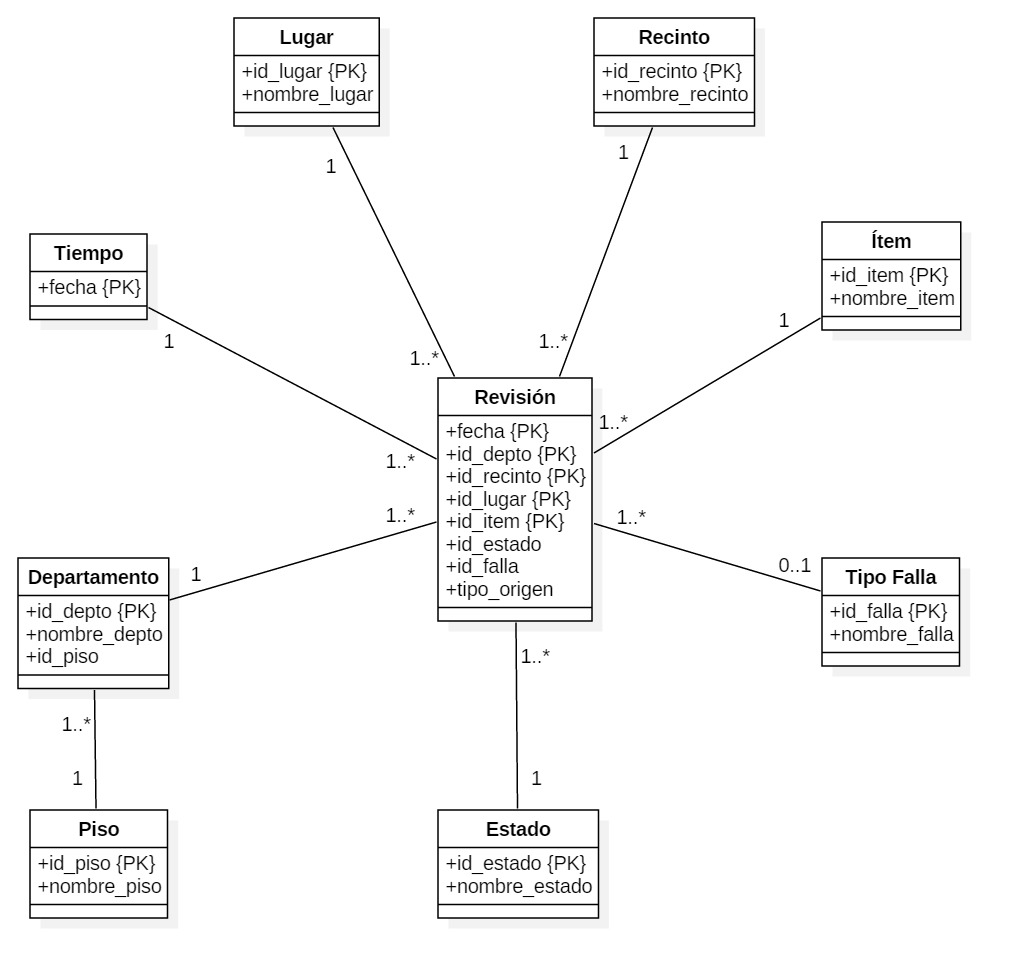
\includegraphics[scale=0.4]{images/Main2.jpg}
\caption{Modelo relacional ROLAP para el proceso de negocio a estudiar.}
\text{Fuente: Elaboración propia}
\label{rolap}
\end{center}
\end{figure}

\section{Aplicación Móvil}
Como se dijo anteriormente, los datos que se utilizarán provienen del módulo “Recepciones” del software CalidadCloud, cuya versión está disponible para plataformas web y dispositivos móviles Android.

Realizando un estudio de la proveniencia de los datos, es decir, desde qué plataforma viene la mayoría de los datos ingresados al sistema, se obtuvo el gráfico mostrado en la Figura \ref{origen}, en la cual se puede observar que un 67,15\% de los datos son ingresados vía móvil, mientras que un 32,85\% se ingresan por web. 

\begin{figure}[H]
\begin{center}
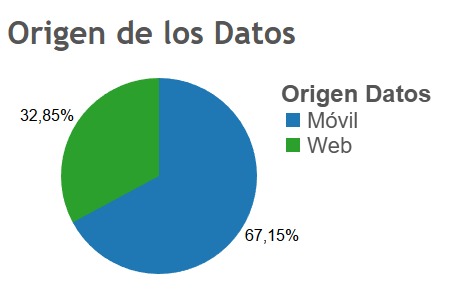
\includegraphics[scale=1]{images/origen.PNG}
\caption{Modelo relacional ROLAP para el proceso de negocio a estudiar.}
\text{Fuente: Elaboración propia}
\label{origen}
\end{center}
\end{figure}

Por lo tanto, en base al análisis, se realizará una mejora a la aplicación, la que constará de un sistema probabilístico básico que permita dar aviso al usuario de las probabilidades que tiene cierto piso, propiedad, recinto, lugar o ítem de fallar, mostrándose en forma de termómetro de falla.

%	IMPLEMENTACIÓN DE LA SOLUCIÓN	------------------------------------------------------------------------------------------------
\newpage
\chapter{Implementación de la Solución}

\section{Herramientas}
\subsection{Tableau}
Tableau\footnote{\url{www.tableau.com}} es un software de origen estadounidense dedicado al análisis de datos. Permite generar una serie de visualizaciones interactivas de los datos que se estudian, poniendo énfasis en la Inteligencia de Negocios.

Tableau permite utilizar datos de diversas fuentes, como son archivos Excel, archivos de texto, servidores MySQL, Amazon, Oracle, Microsoft, entre otros.

Cuando los datos son cargados al software, éste muestra todas las dimensiones y medidas que se pueden utilizar para su análisis, arrastrándolas hacia una hoja de trabajo en donde se puede modificar los datos a mostrar, el tipo de gráfico o información que se desea presentar de acuerdo al negocio y propósito. 

Existen diversos tipos de gráficos y paletas de colores, lo que permite al usuario poder utilizar el que mejor represente el resultado del análisis realizado. Con esto, se pueden crear dashboards y libros de historia en donde se van mostrando los gráficos y la información para que los interesados puedan observarlos de forma intuitiva y eficaz.

Tableau ha obtenido múltiples premios y reconocimientos. El último le fue dado en el año 2015 por ser el software \#1 en “ability to execute” y el líder en “completeness in vision”, premios que fueron entregados por la consultora Gartner, Inc. en Magic Quadrant for Business Intelligence and Analytics Platforms \cite{magic}. La figura \ref{gartner} muestra el resultado del análisis de Gartner para el año 2016, en donde se puede ver que Tableau sigue siendo líder de entre todos los softwares de análisis de datos y BI.

\begin{figure}[H]
\begin{center}
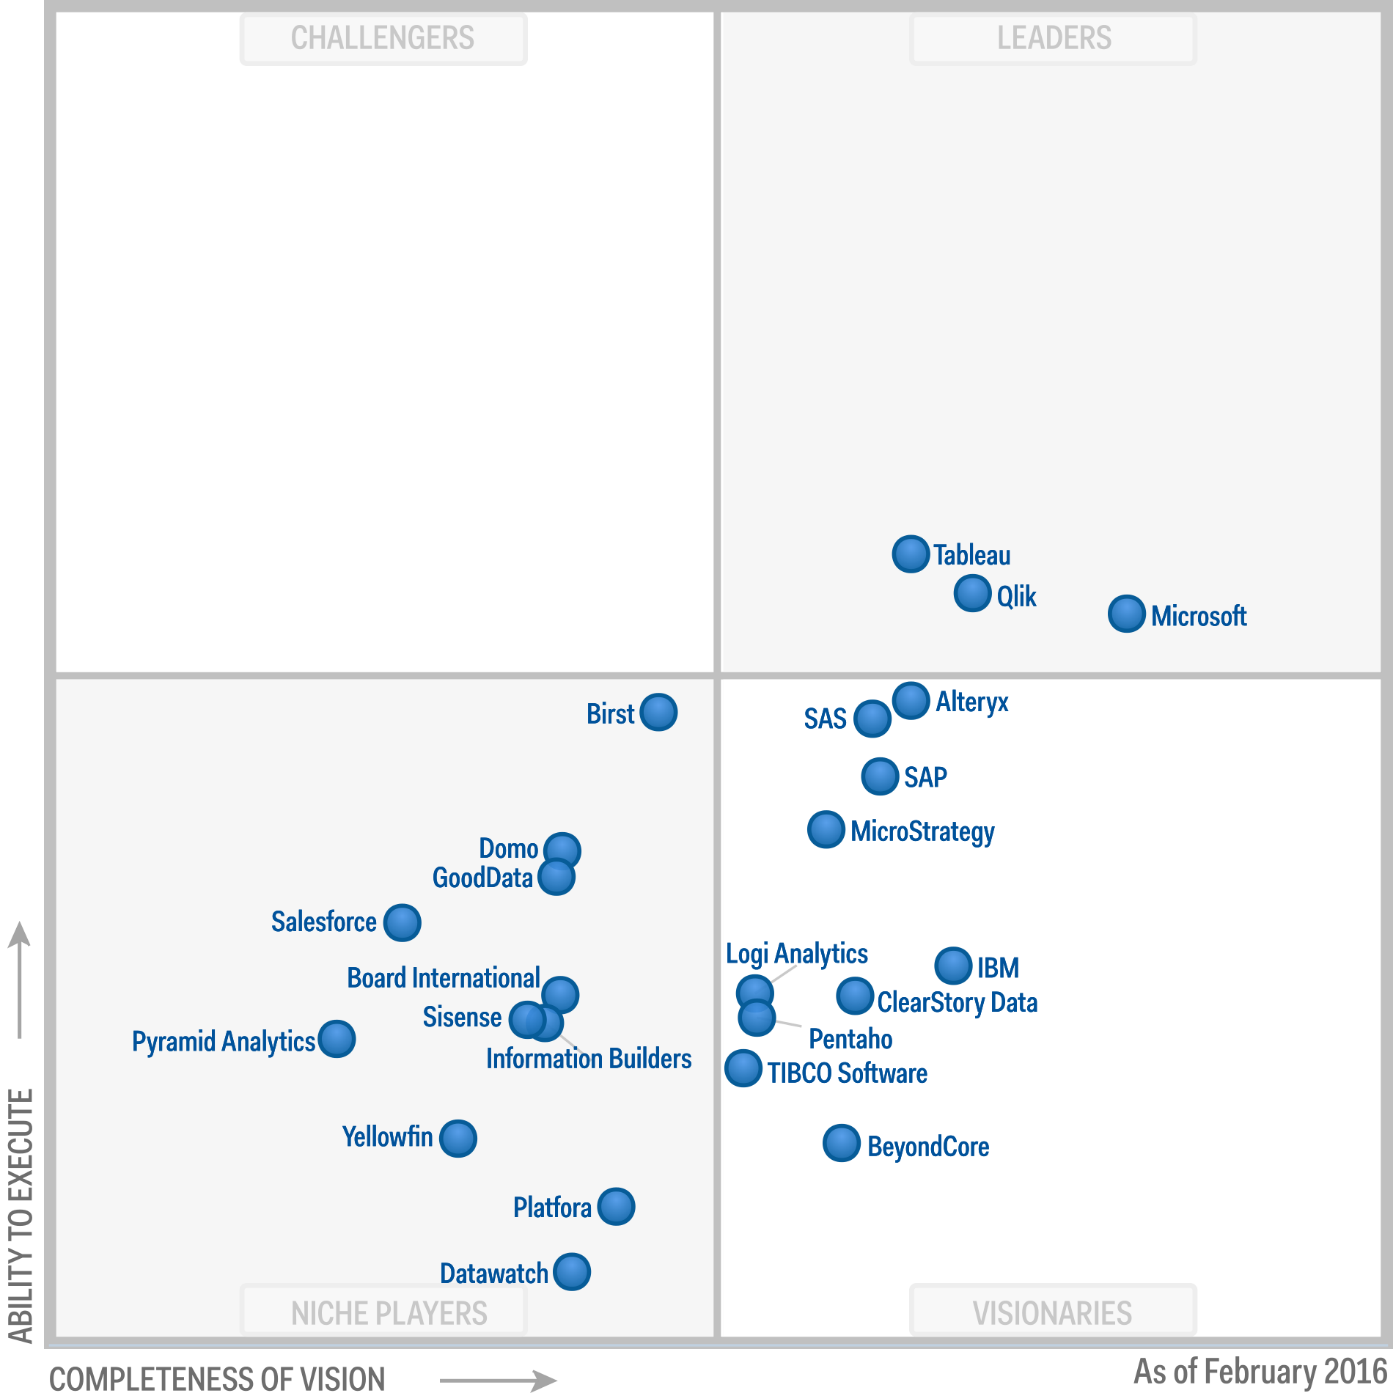
\includegraphics[scale=0.7]{images/gartner.PNG}
\caption{Cuadrante Mágico para plataformas de Inteligencia de Negocios}
\text{Fuente: \cite{magic}}
\label{gartner}
\end{center}
\end{figure}
Tableau es un completo software que permite trabajar con Big Data\footnote{Big Data: enormes cantidades de datos que tomaría demasiado tiempo y sería muy costoso cargarlos a un base de datos relacional para su análisis \cite{bigdata}} en tiempo real o en memoria, para facilitar su visualización en equipos portátiles. Además, dentro de sus funcionalidades, está detectar tendencias e identificar oportunidades de negocio que no son visibles a primera vista, lo que genera valor a la empresa. En general, tiene todas las características que facilitan el análisis de datos, haciéndolo simple y entendible por cualquier persona.

\subsection{PhoneGap}
PhoneGap\footnote{\url{www.phonegap.com}} es un framework open source que permite desarrollar aplicaciones móviles usando tecnologías web. Simplifica la tarea de desarrollar aplicaciones exclusivamente para Android o iOS en los lenguajes Java y Objective C respectivamente, de tal forma que con un solo click se pueda construir la misma aplicación para ambos sistemas operativos sin perder tiempo en desarrollar cada una en su respectivo lenguaje.

Este framework, pertenece a la empresa Adobe, dueña de múltiples softwares de uso profesional y de escritorio. Es utilizada por muchos desarrolladores y muchas aplicaciones están hechas en base a esta tecnología, incluyendo la app “Recepciones”, desde la cual se obtuvieron los datos que se analizarán.

La aplicación “Recepciones” hecha con PhoneGap, está desarrollada con el lenguaje PHP, Javascript y JQuery. Se utilizará un Smartphone con sistema operativo Android 5.0 para probar los resultados que se obtengan durante el desarrollo de las alertas de falla en la revisión de propiedades.

\subsubsection{Funcionamiento}
Phonegap genera una estructura en la cual se puede desarrollar una página en HTML5, Javascript y CSS que luego usara dentro de una aplicación predefinida. Esta aplicación embeberá el código HTML en un componente del sistema operativo: UIWebView (iOS) y WebView (Android). Como suele suceder en estos casos, el componente tiene, por seguridad, muchas restricciones de acceso al sistema operativo y hardware del dispositivo. \cite{phonegap}

Para contrarrestar estas limitaciones, Phonegap ofrece un sistema modular que permite el registro de plugins. Este sistema modular es llamado bridge (puente) y se encarga de generar una interfaz entre el codigo Javascript corriendo en el componente web y las llamadas a funcionalidades nativas del sistema operativo. La arquitectura de PhoneGap se puede ver en la Figura \ref{phonegap}.

\begin{figure}[H]
\begin{center}
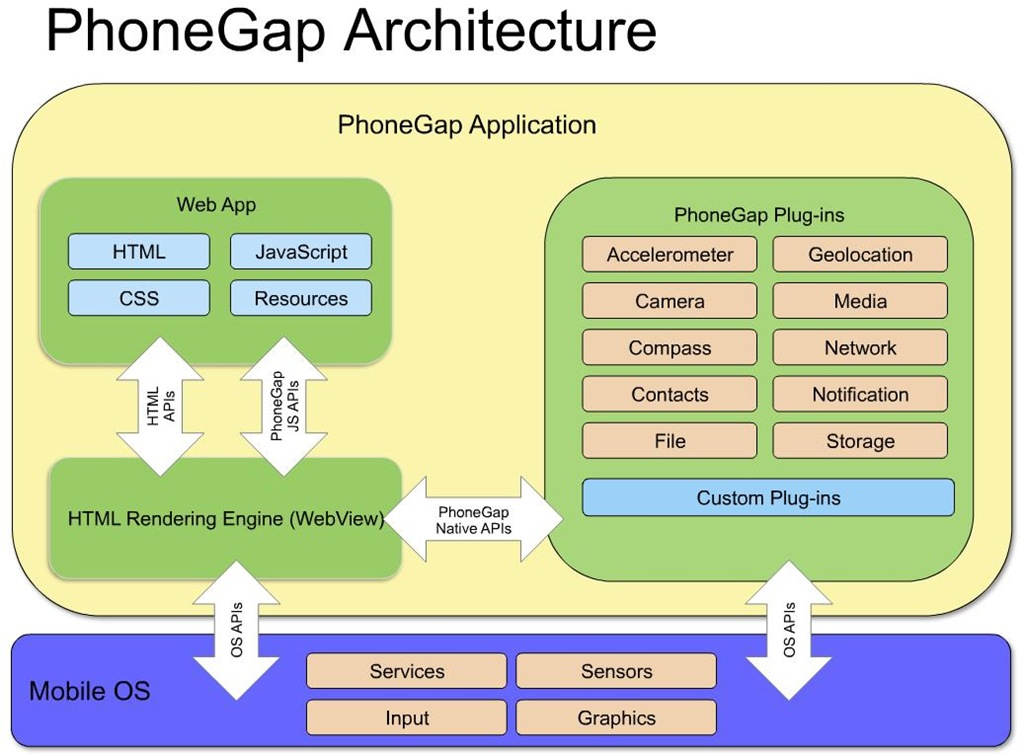
\includegraphics[scale=0.5]{images/phonegap.jpg}
\caption{Cuadrante Mágico para plataformas de Inteligencia de Negocios}
\text{Fuente: \cite{phonegap}}
\label{phonegap}
\end{center}
\end{figure}

\section{Visualización de los Resultados}
Para visualizar los resultados obtenidos en el análisis OLAP, se crearon una serie de gráficos y dashboards que ayudarán a comprender de una forma fácil las tendencias y características actuales de los datos.

En Tableau, se importaron los datos desde los archivos .csv de cada empresa y se realizó una unión de los archivos, para tener un análisis industrial y global de los datos. Luego, al tener todas las dimensiones necesarias para responder a los requerimientos especificados en la sección anterior, se comienza a realizar análisis OLAP, generando distintos tipos de gráficos que respondan lo esperado.

\section{Termómetro de fallas en App}
ACA detalle de cómo se programó la aplicación

%	ANÁLISIS Y RESULTADOS		-----------------------------------------------------------------------------------------------------------
\newpage
\chapter{Análisis y Resultados}
Los datos que se estudiarán y que se utilizaron para realizar el análisis OLAP, fueron recolectados entre el 31 de diciembre del 1999 y 03 de enero del año 2000, saltándose al 21 de septiembre del 2015 hasta el 10 de agosto del 2016.

Anteriormente, no se han hecho análisis de los datos recopilados por la aplicación, por lo que este sería el primer acercamiento a conocer el estado de la industria en Chile.

El objetivo de esta memoria, es hacer un estudio sobre las fallas más frecuentes en las terminaciones de las propiedades en Chile, analizando sobre varias dimensiones y variables que permitan conocer tendencias o patrones. 

\section{Fallas en Recintos, Lugares e Ítems}
A continuación, se muestra una imágen con los recintos, lugares e ítems que más fallas presentan en el sistema.
\begin{figure}[H]
\begin{center}
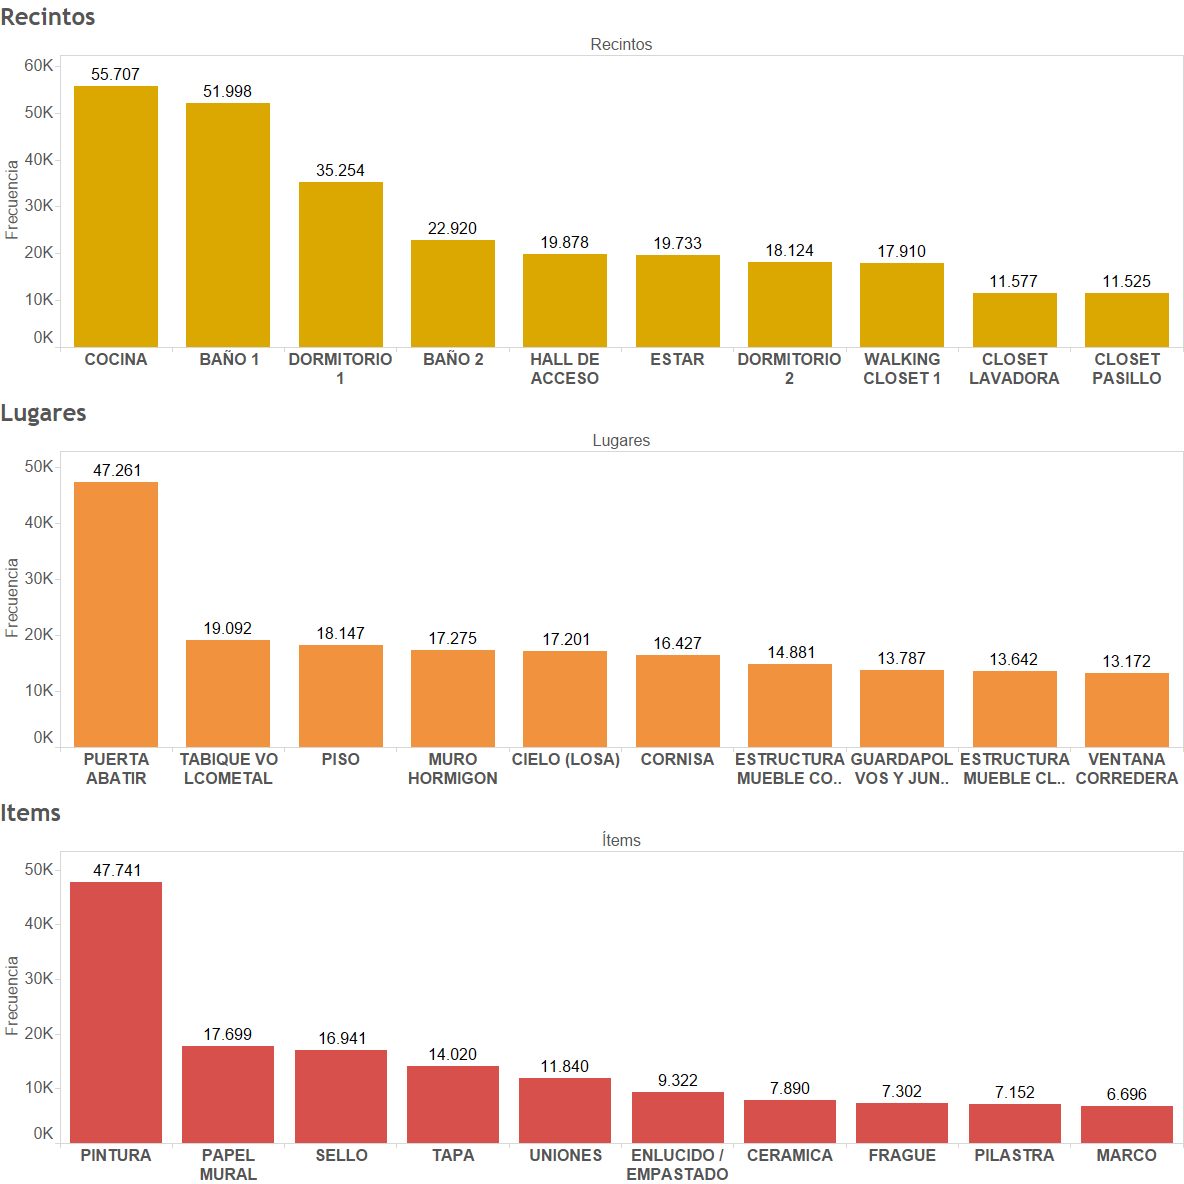
\includegraphics[scale=0.7]{images/Dashboard1.png}
\caption{Cuadrante Mágico para plataformas de Inteligencia de Negocios}
\text{Fuente: Elaboración propia}
\label{}
\end{center}
\end{figure}

En la siguiente imágen se muestran los recintos que más fallas, con sus respectivos lugares e ítems en que presentan los problemas.

\begin{figure}[H]
\begin{center}
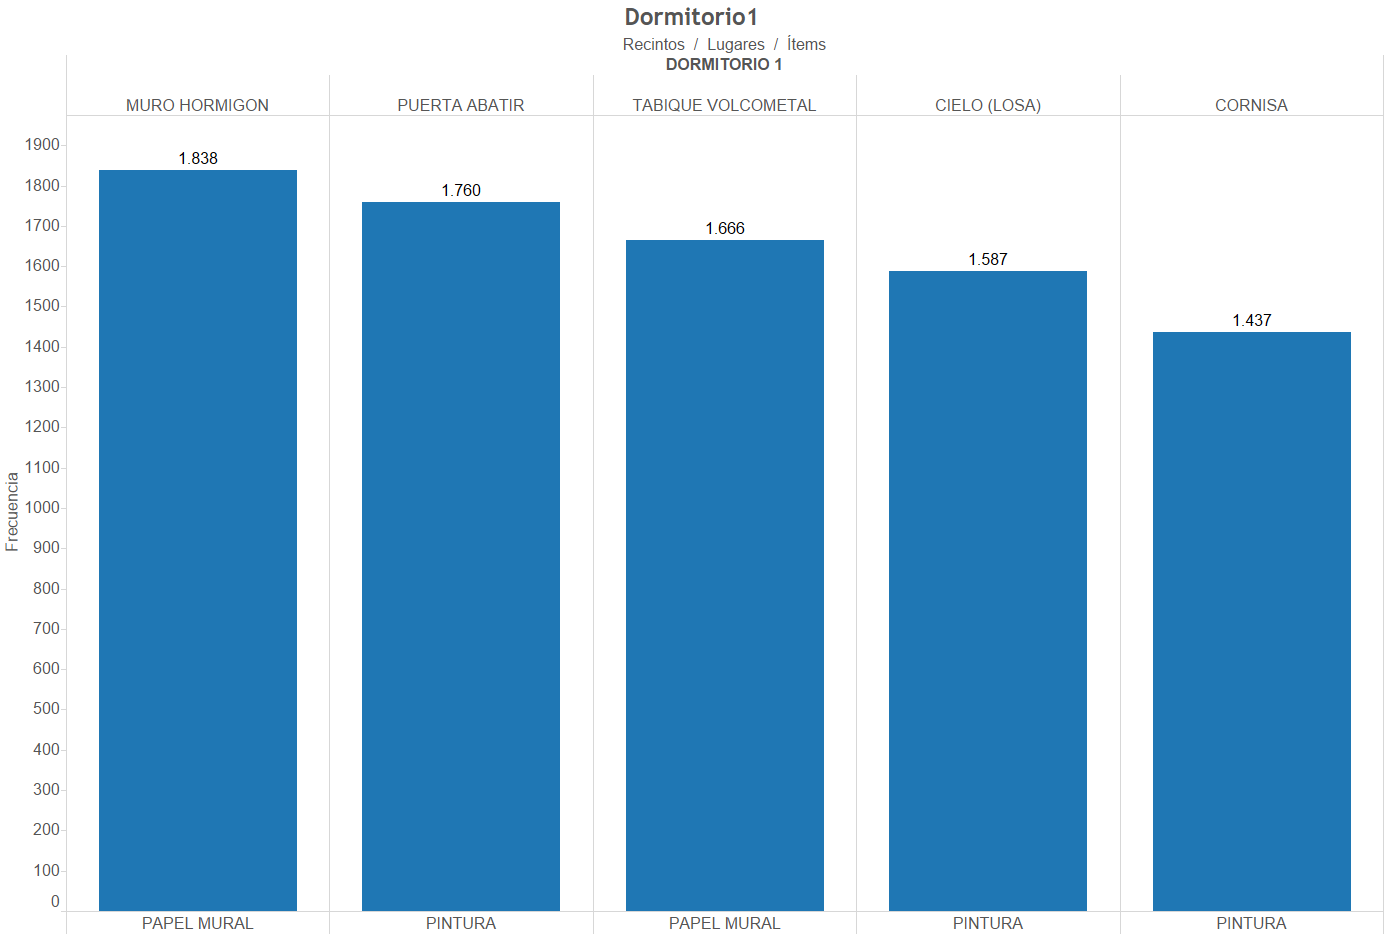
\includegraphics[scale=0.5]{images/Dormitorio1.png}
\caption{Fallas en recinto DORMITORIO 1}
\text{Fuente: Elaboración propia}
\label{}
\end{center}
\end{figure}

\begin{figure}[H]
\begin{center}
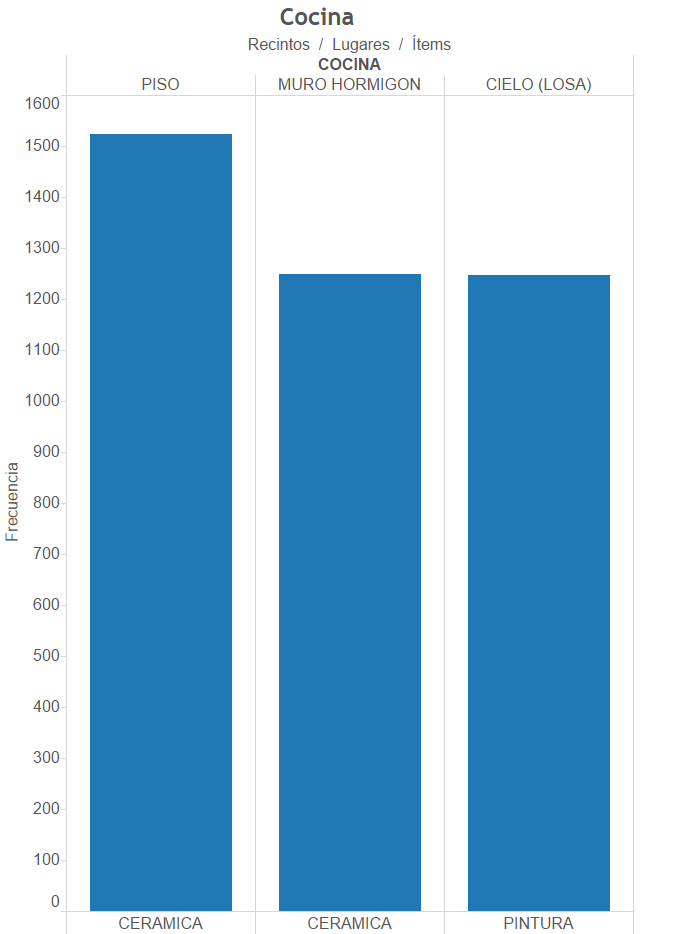
\includegraphics[scale=0.5]{images/cocina.png}
\caption{Fallas en recinto COCINA}
\text{Fuente: Elaboración propia}
\label{}
\end{center}
\end{figure}

\begin{figure}[H]
\begin{center}
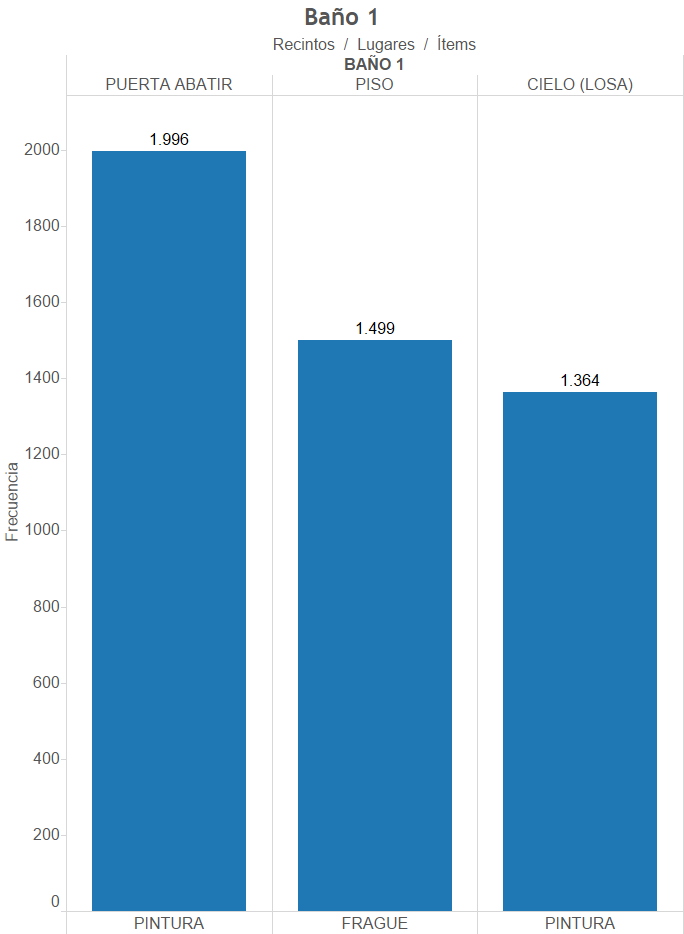
\includegraphics[scale=0.5]{images/bano1.png}
\caption{Fallas en recinto BAÑO 1}
\text{Fuente: Elaboración propia}
\label{}
\end{center}
\end{figure}

\begin{figure}[H]
\begin{center}
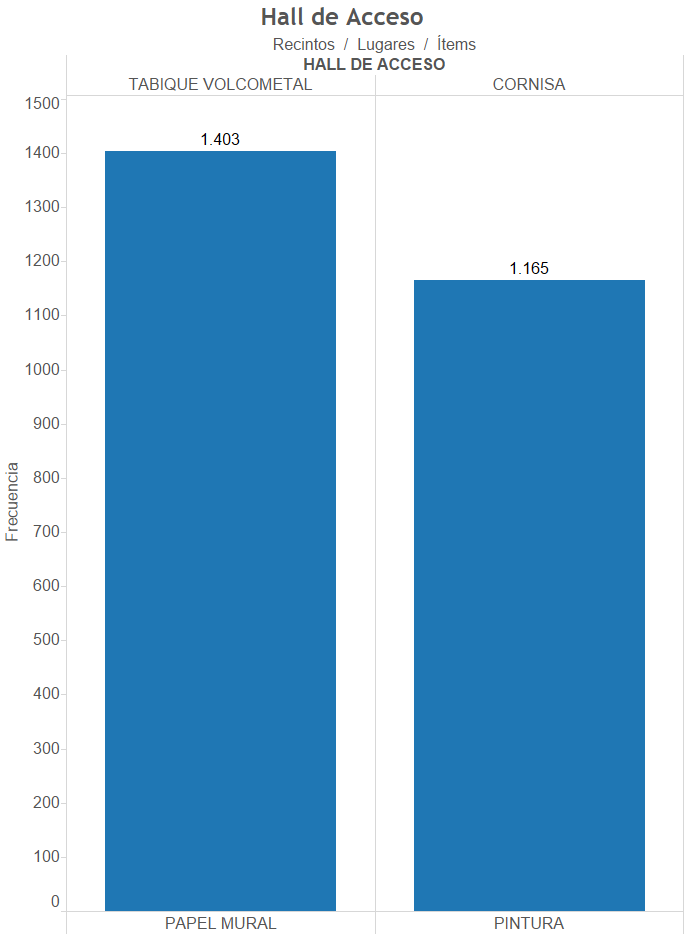
\includegraphics[scale=0.5]{images/hall.png}
\caption{Fallas en recinto HALL DE ACCESO}
\text{Fuente: Elaboración propia}
\label{}
\end{center}
\end{figure}

\begin{figure}[H]
\begin{center}
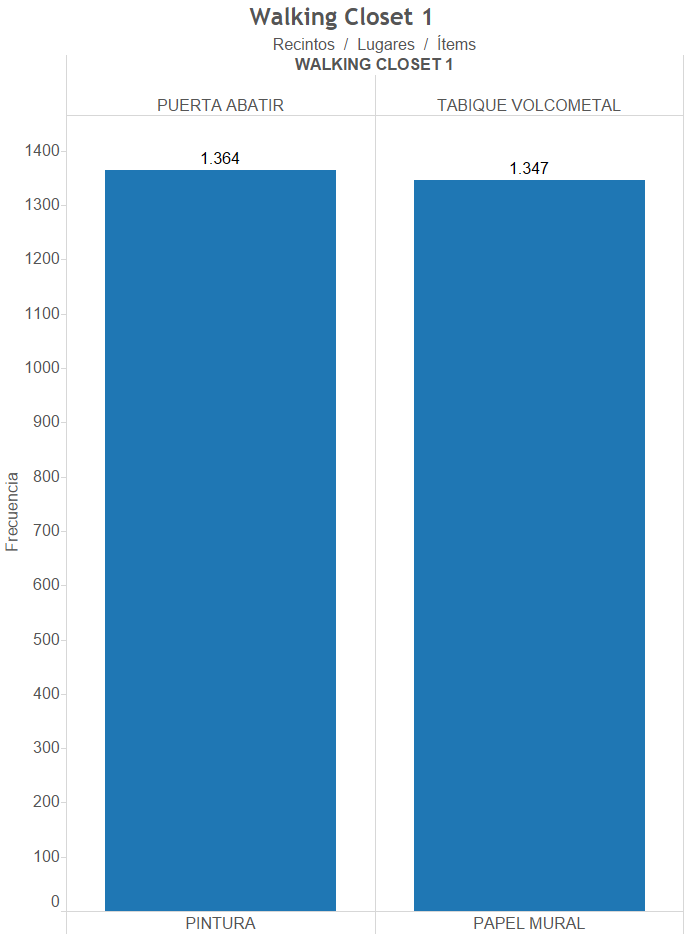
\includegraphics[scale=0.5]{images/walking.png}
\caption{Fallas en recinto WALKIN CLOSET 1}
\text{Fuente: Elaboración propia}
\label{}
\end{center}
\end{figure}

\begin{figure}[H]
\begin{center}
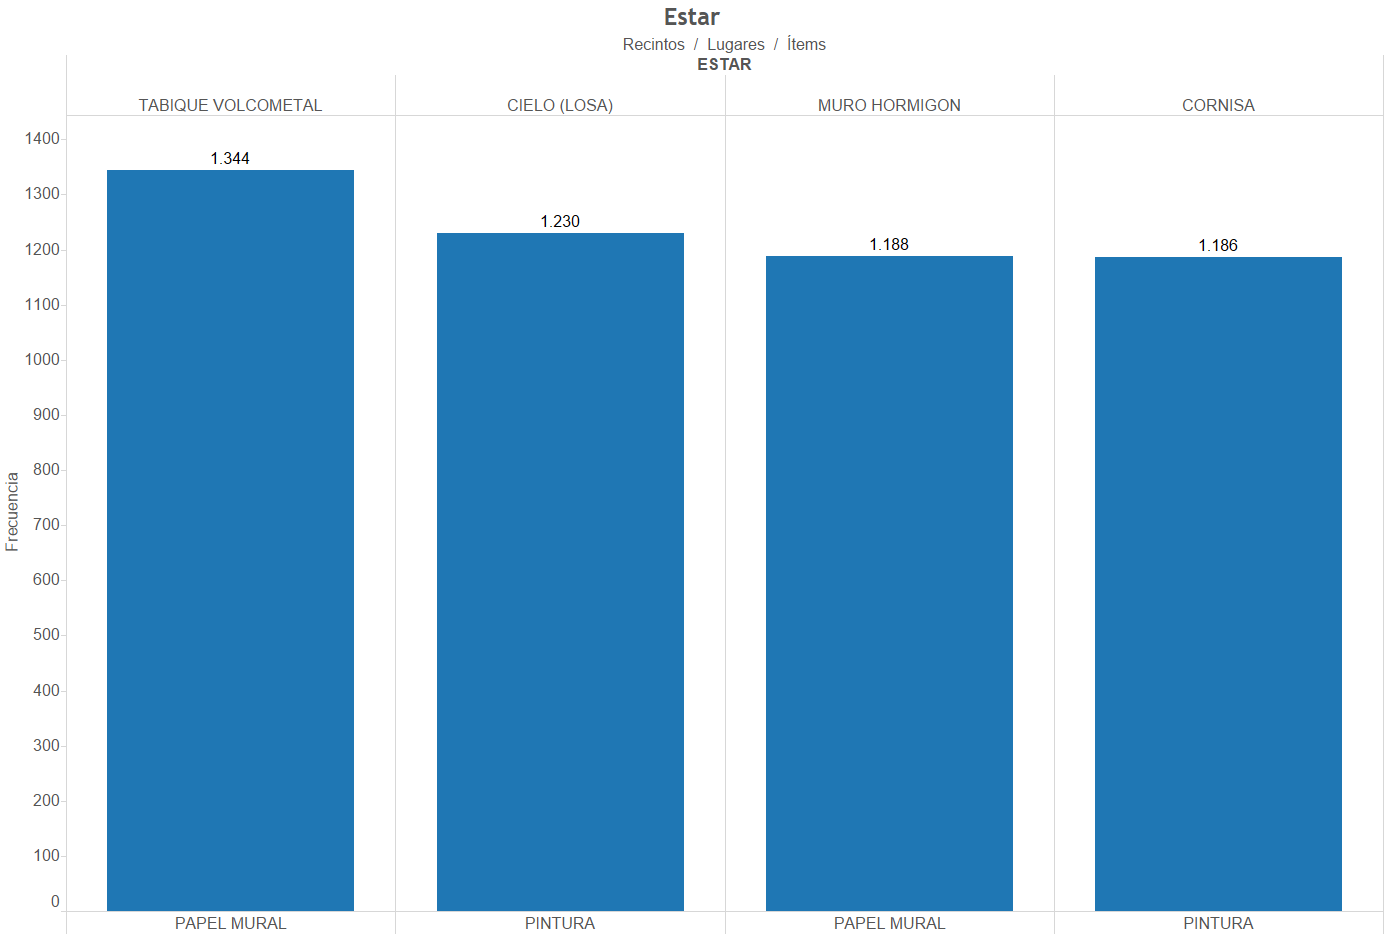
\includegraphics[scale=0.5]{images/estar.png}
\caption{Fallas en recinto ESTAR}
\text{Fuente: Elaboración propia}
\label{}
\end{center}
\end{figure}

\section{Tipos de Fallas}
Se muestran los tipos de fallas más frecuentes en las revisiones, independientemente del recinto, lugar o ítem en donde ocurren.
\begin{figure}[H]
\begin{center}
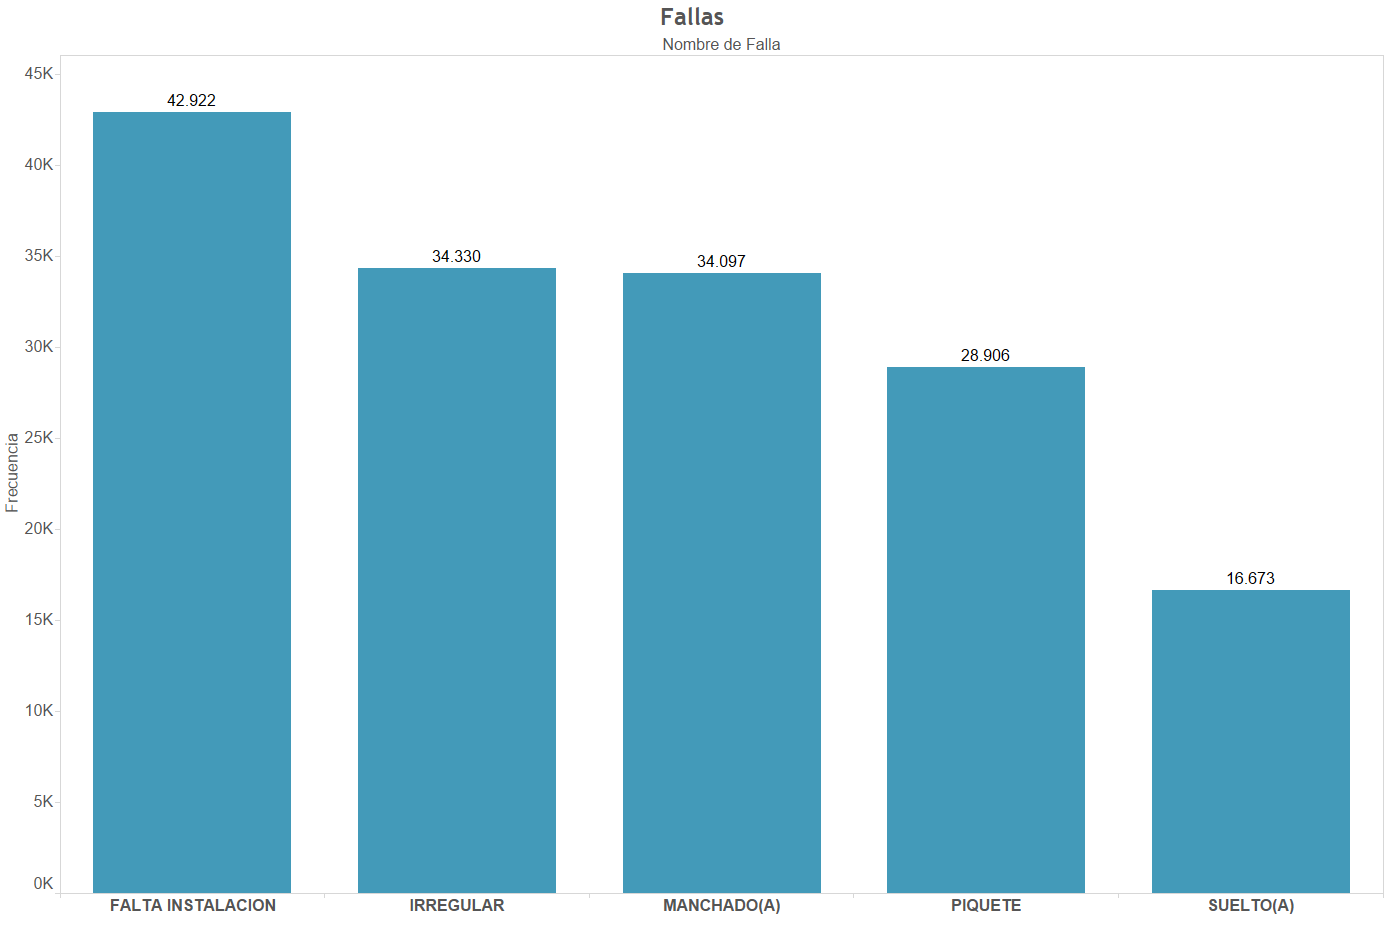
\includegraphics[scale=0.7]{images/tipos_fallas.png}
\caption{Tipos de fallas más comunes}
\text{Fuente: Elaboración propia}
\label{}
\end{center}
\end{figure}

En la siguiente figura se muestran los tipos de fallas que presentaban los recintos con más fallas.
\begin{figure}[H]
\begin{center}
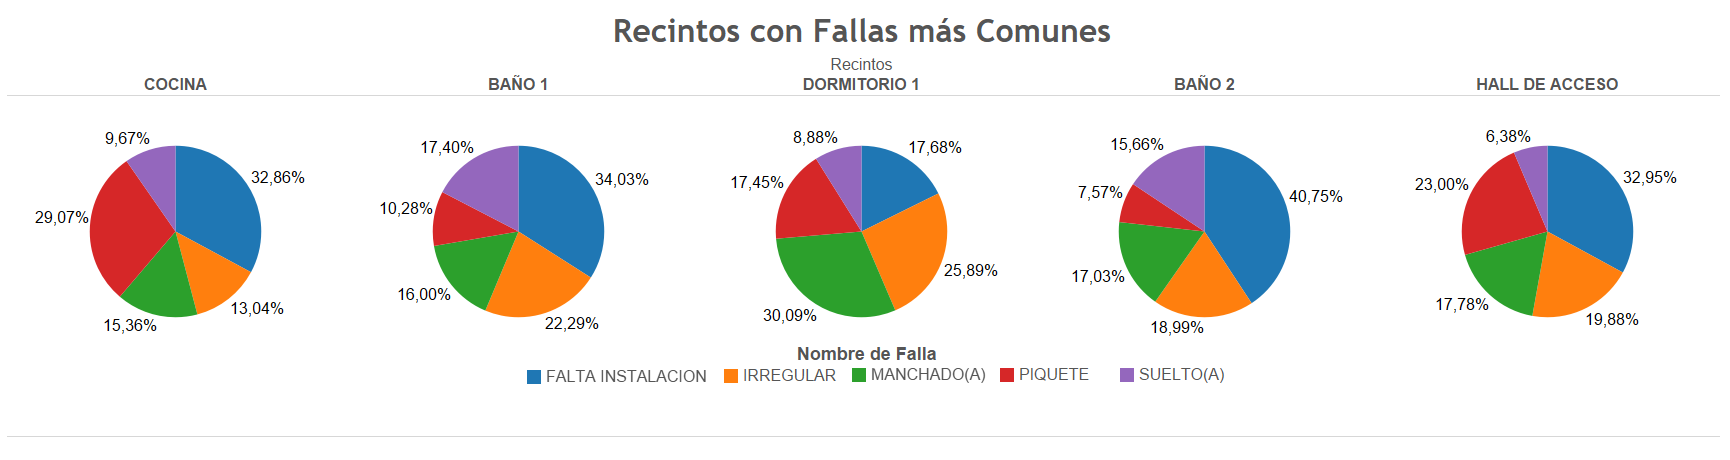
\includegraphics[scale=0.5]{images/recintos_fallas.png}
\caption{Recintos con fallas más comunes}
\text{Fuente: Elaboración propia}
\label{}
\end{center}
\end{figure}

En la siguiente figura se muestran los tipos de fallas que presentaban los lugares con más fallas.
\begin{figure}[H]
\begin{center}
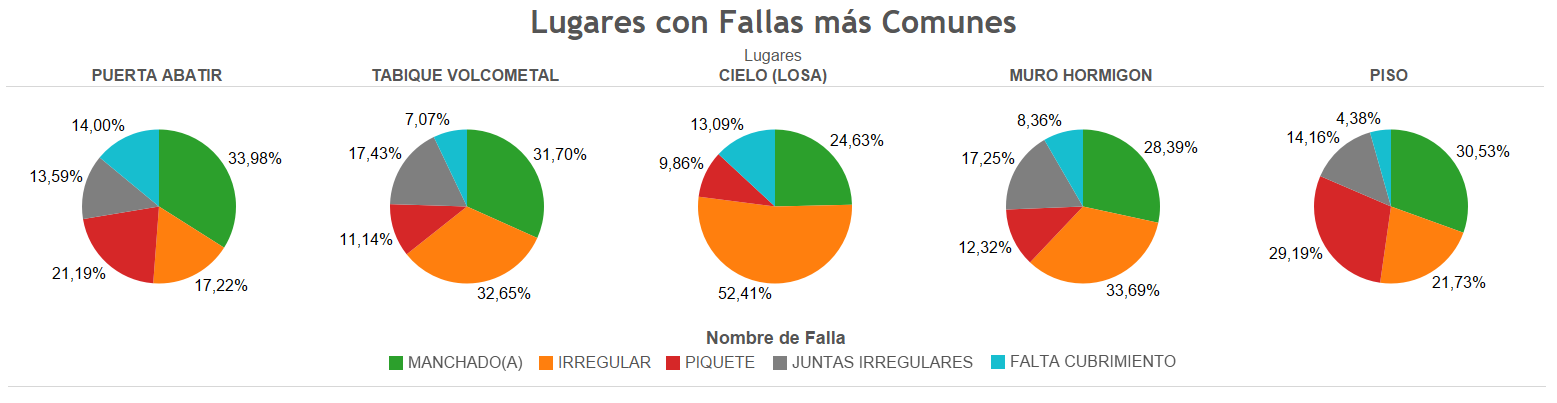
\includegraphics[scale=0.56]{images/lugares_fallas.png}
\caption{Lugares con fallas más comunes}
\text{Fuente: Elaboración propia}
\label{}
\end{center}
\end{figure}

En la siguiente figura se muestran los tipos de fallas que presentaban los ítems con más fallas.

\begin{figure}[H]
\begin{center}
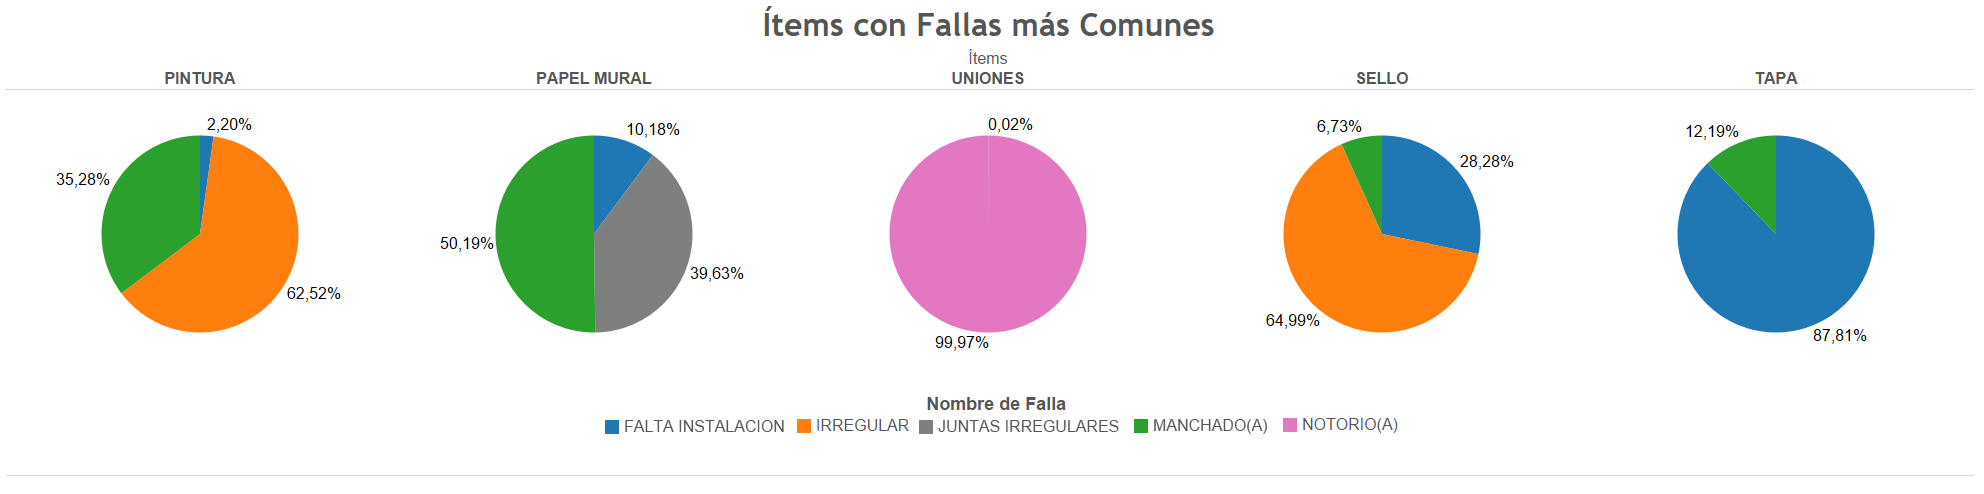
\includegraphics[scale=0.44]{images/items_fallas.png}
\caption{Ítems con fallas más comunes}
\text{Fuente: Elaboración propia}
\label{}
\end{center}
\end{figure}

\section{Fallas por Piso}
A continuación, se muestra la cantidad de fallas por piso.
\begin{figure}[H]
\begin{center}
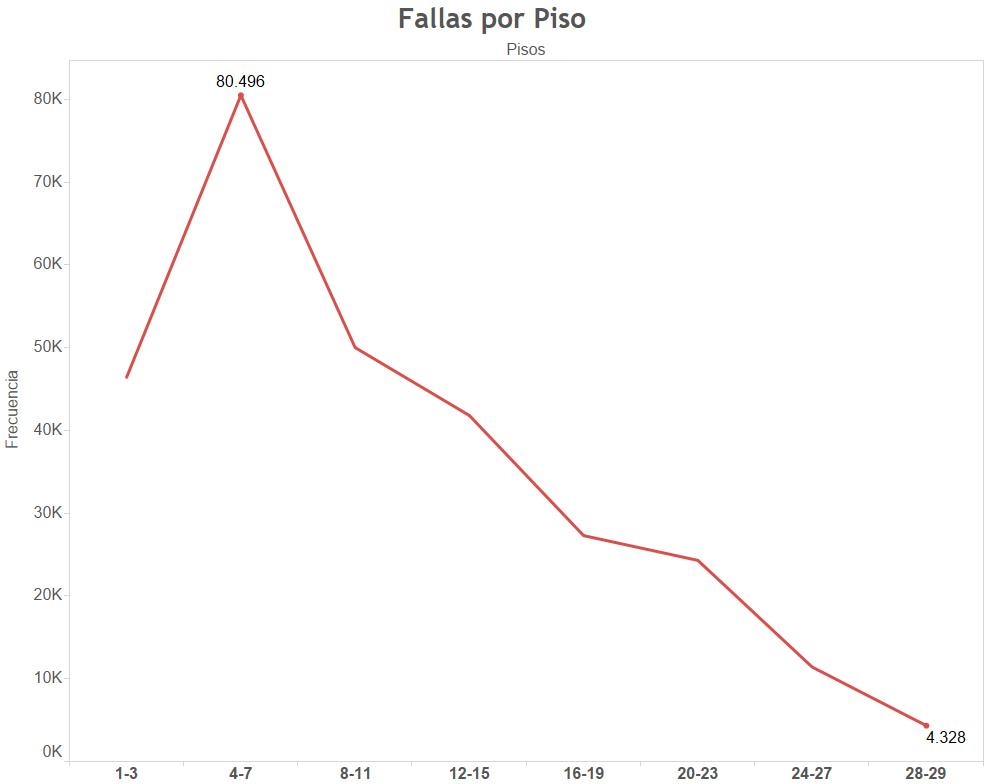
\includegraphics[scale=0.7]{images/fallas_piso.png}
\caption{Fallas por piso}
\text{Fuente: Elaboración propia}
\label{}
\end{center}
\end{figure}

%	CONCLUSIONES	---------------------------------------------------------------------------------------------------------------------------

%	ANEXOS		--------------------------------------------------------------------------------------------------------------------------------

%	REFERENCIAS	---------------------------------------------------------------------------------------------------------------------------
\newpage
\fancyhf{}
\lhead{\leftmark}
\fancyfoot[R]{\thepage}
\addcontentsline{toc}{section}{Referencias Bibliográficas}
%\begin{thebibliography}{[MT1]}
\bibliographystyle{plain}
\bibliography{Referencias}

%\end{thebibliography}
\end{document} 
